\section{Design Overview}

The Fire Alarm Notification System (FANS) is a real-time system designed for efficient fire detection and alerting. The
system is composed of several key components, each with a distinct function but integrated to work seamlessly together,
ensuring a comprehensive approach to fire safety. The system's architecture is outlined in a detailed deployment
diagram in Figure \ref{fig:deployment}, illustrating the interconnections between the various components. These
components include:

\begin{itemize}
    \item \textbf{Alarm System:} Based on a Raspberry Pi 4, this system triggers audible and visual alerts in the event
          of a fire, ensuring that occupants are promptly warned.

    \item \textbf{Smoke Detection System:} Also utilizing a Raspberry Pi 4, this system constantly monitors the
          environment for smoke using advanced sensors. It is the primary detection mechanism that activates the alarm
          system and notification system upon detecting smoke.

    \item \textbf{Notification System:} Operating on a Raspberry Pi 4, this system sends out emergency alerts to
          predefined contacts, including both local authorities and individuals, ensuring rapid response to the detected
          fire.

    \item \textbf{Cloud Database:} A real-time cloud database is employed to store critical data, including sensor
          readings (smoke and temperature levels) and system configurations. This facilitates remote monitoring and
          configuration, ensuring that the system is always functioning optimally.

    \item \textbf{Haptic Alarm:} This device provides haptic feedback, offering an additional layer of alert through
          physical sensation, ensuring that even those who may not be within hearing range of the alarm or have hearing
          impairments are alerted.

    \item \textbf{User Interface:} A web-based application for monitoring the system's environment and configuring
          system settings.
\end{itemize}

The system's design emphasizes scalability, allowing for easy expansion with additional sensors or alarm units as
needed. It also highlights modularity, where each component can function independently, ensuring reliability and ease
of maintenance. Communication between the components is facilitated through a local network, with the cloud database
supporting remote access and control.

Furthermore, the system incorporates advanced communication protocols for efficient data exchange and alerting. The
smoke detection system employs the I2C protocol for sensor communication, while UDP packets facilitate local network
communication between the system's nodes. HTTP requests are utilized for interactions with the cloud-hosted real-time
Firebase database, ensuring timely updates and access to system data.

Overall, the Fire Alarm Notification System is designed to be a reliable, efficient, and scalable solution for fire
detection and notification, leveraging modern technology to provide real-time alerts and ensuring the safety of
occupants in any building.

\subsection{System Overview Design}

\begin{figure}[H]
    \centering
    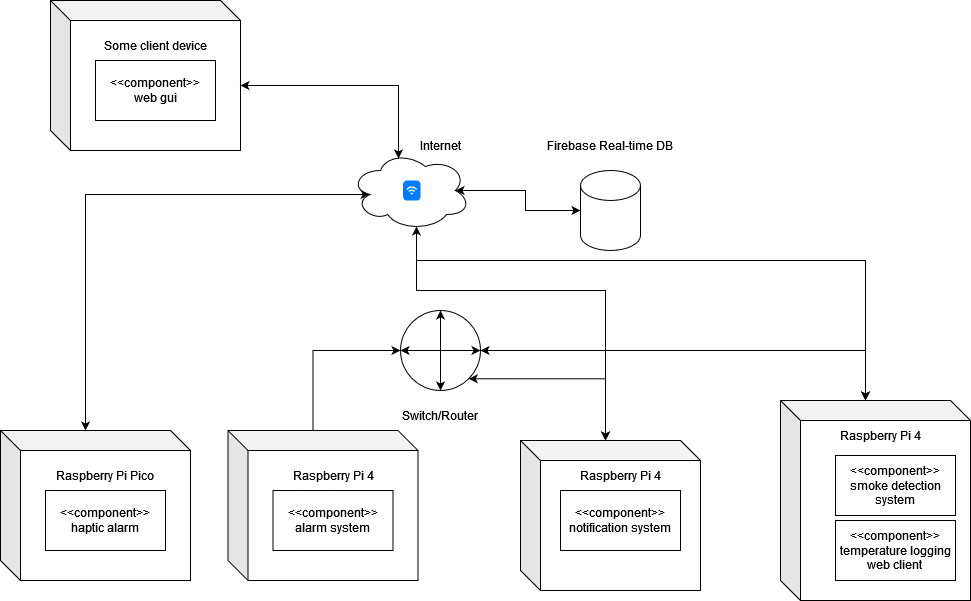
\includegraphics[width=\linewidth]{../assets/FANSDeployment.png}
    \caption{The deployment diagram for FANS.}
    \label{fig:deployment}
\end{figure}

\subsection{Communication Protocols}

In the Fire Alarm Notification System (FANS), a variety of communication protocols are meticulously integrated to
ensure seamless interaction among the system components and with the external cloud database, facilitating a robust and
responsive fire alarm solution.

The system's core, the Smoke Detection System, communicates with its temperature and smoke sensors using the I2C
protocol over the GPIO pins of a Raspberry Pi 4. This protocol choice is pivotal for real-time data acquisition,
allowing the system to monitor environmental conditions continuously and detect any signs of fire immediately. For
interactions within the local network, including communication between the smoke detection system, the alarm system,
and the notification system, UDP packets are employed. This approach is selected for its efficiency and speed, ensuring
that critical data is transmitted quickly and reliably across the system components without the overhead of
establishing and maintaining a connection, which is crucial in emergency situations where every second counts.

The integration with the cloud is achieved through HTTP requests to a Firebase real-time database. This cloud database
is essential for storing sensor data, system configurations, and user information. It supports various operations,
including the posting of sensor data by the smoke detection system, retrieval of data for the web GUI, fetching contact
information for the notification system, and polling for emergency flags by the haptic alarm system. These interactions
are facilitated by HTTP's flexibility and its widespread support across internet infrastructure, enabling the FANS to
leverage cloud computing benefits for enhanced data management and accessibility.

Lastly, the notification system's ability to reach users through email and SMS text notifications is realized through
standard internet SMS and email protocols. This ensures that in the event of a fire, users are promptly informed
regardless of their location, providing critical information and instructions to enhance their safety and response
effectiveness.

Together, these communication protocols form the backbone of the Fire Alarm Notification System, enabling it to
function as a cohesive, efficient, and highly responsive fire safety solution.

The Fire Alarm Notification System (FANS) employs a variety of communication protocols to ensure seamless interactions
between its components and with the external cloud database. This section provides detailed tables describing each
communication pathway.

\subsubsection{I2C Communication}

The Raspberry Pi 4 utilizes the I2C protocol to communicate with an array of temperature and smoke sensors, monitoring
environmental conditions to detect potential fire hazards. This is not visible in the sequence diagrams as they show
the bigger picture of the communication of the nodes with the sensors.

\begin{table}[H]
    \centering
    \begin{tabular}{| c | c | c | c | c |}
        \hline
        Sender         & Receiver               & Message              & Data Format                                          & Protocol                 \\
        \hline
        Raspberry Pi 4 & Temperature Sensor     & \texttt{read\_temp}  & See section 6.2.1 of datasheet \cite{temp-datasheet} & I2C                      \\
        \hline
        Raspberry Pi 4 & Smoke Sensor (via ADC) & \texttt{read\_smoke} & See figure 1.1 of datasheet \cite{adc-datasheet}     & SPI \cite{adc-datasheet} \\
        \hline
    \end{tabular}
    \caption{Messages for I2C communication in FANS.}
\end{table}

\subsubsection{Local Area Network Communication}

Nodes within the FANS (smoke detection, alarm, and notification systems) communicate over a local network using UDP
packets, facilitating real-time alerts and system coordination.

The messages sent over UDP use numerical value to encode messages. The representation agreed upon is as follows:

\begin{table}[H]
    \centering
    \begin{tabular}{| c | c |}
        \hline
        Message      & Value \\
        \hline
        Emergency    & 0     \\
        \hline
        No Emergency & 1     \\
        \hline
    \end{tabular}
    \caption{Numerical representation of messages over UDP in FANS.}
\end{table}

\begin{table}[H]
    \centering
    \begin{tabular}{| c | c | c | c | c |}
        \hline
        Sender                 & Receiver            & Message      & Data Format & Protocol \\
        \hline
        Smoke detection system & Notification system & Emergency    & 0           & UDP      \\
        \hline
        Smoke detection system & Alarm system        & Emergency    & 0           & UDP      \\
        \hline
        Smoke detection system & Notification system & No emergency & 1           & UDP      \\
        \hline
        Smoke detection system & Alarm system        & No Emergency & 1           & UDP      \\
        \hline
    \end{tabular}
    \caption{Messages for local area network communication in FANS.}
\end{table}

\subsubsection{Cloud Database Communication}

\begin{table}[H]
    \centering
    \begin{tabular}{| c | c | c | c | c |}
        \hline
        Sender          & Receiver & Message                                    & Data Format                      & Protocol    \\
        \hline
        Smoke Detection & Cloud DB & \texttt{put\_sensor\_data()}               & See listing \ref{lst:sensor}     & HTTP (JSON) \\
        \hline
        GUI             & Cloud DB & \texttt{update\_threshold(new\_threshold)} & See listing \ref{lst:threshold}  & HTTP (JSON) \\
        \hline
        Notification    & Cloud DB & \texttt{query\_contact\_information()}     & See listing \ref{lst:contact}    & HTTP (JSON) \\
        \hline
        Haptic Alarm    & Cloud DB & \texttt{emergency()}                       & See listing \ref{lst:emergency}  & HTTP (JSON) \\
        \hline
        GUI             & Cloud DB & \texttt{get\_sensor\_data()}               & See listing \ref{lst:sensor-get} & HTTP (JSON) \\
        \hline
    \end{tabular}
    \caption{Messages for cloud database communication in FANS.}
\end{table}

\begin{lstlisting}[language=json,label={lst:sensor},caption={Update sensor data message.}]
{
  "method": "PUT",
  "path": "/sensor-data/temperature",
  "headers": {
    "Authorization": "Bearer YOUR_ACCESS_TOKEN",
    "Content-Type": "application/json"
  },
  "body": {
      "data": {
          "temperature": 21.2,
          "timestamp": "2024-03-13T08:37:22"
      }
  }
}
\end{lstlisting}

\begin{lstlisting}[language=json,label={lst:threshold},caption={Threshold update message.}]
{
  "method": "PUT",
  "path": "/system/threshold",
  "headers": {
    "Authorization": "Bearer YOUR_ACCESS_TOKEN",
    "Content-Type": "application/json"
  },
  "body": {
    "newThreshold": 50
  }
}
\end{lstlisting}

\begin{lstlisting}[language=json,label={lst:contact},caption={Request for user contact information.}]
{
  "method": "GET",
  "path": "/user/contact",
  "headers": {
    "Authorization": "Bearer YOUR_ACCESS_TOKEN"
  }
}
\end{lstlisting}

\begin{lstlisting}[language=json,label={lst:emergency},caption={Request for emergency flag.}]
{
  "method": "GET",
  "path": "/system/emergency",
  "headers": {
    "Authorization": "Bearer YOUR_ACCESS_TOKEN"
  }
}
\end{lstlisting}

\begin{lstlisting}[language=json,label={lst:sensor-get},caption={Request for latest sensor data.}]
{
  "method": "GET",
  "path": "/sensor-data",
  "headers": {
    "Authorization": "Bearer YOUR_ACCESS_TOKEN"
  }
}
\end{lstlisting}

\subsubsection{User Notification Communication}

The notification system communicates with users through email, employing standard internet protocols to ensure timely
and effective alerts.

\begin{table}[H]
    \centering
    \begin{tabular}{| c | c | c | c | c |}
        \hline
        Sender              & Receiver   & Message                & Data Format                 & Protocol     \\
        \hline
        Notification System & User Inbox & Emergency notification & See listing \ref{lst:email} & SMTP (Email) \\
        \hline
    \end{tabular}
    \caption{Messages for user notification communication in FANS.}
\end{table}

\begin{lstlisting}[label={lst:email},caption={Email notification for detected emergency in FANS.}]
FROM: notification@example.com
TO: user@example.com
SUBJECT: Fire Alarm Notification

Dear [User's Name],

Fire alarm detected. Evacuate immediately.

- Location: [Location]
- Date/Time: [Date/Time]

Stay safe!
\end{lstlisting}

\subsection{Message Sequence Diagrams}

To implement the functional requirements described in Section 1.1: Functional Requirements, the FANS system will
satisfy six core use cases highlighted and illustrated in the message sequence diagrams below.

\subsubsection{Trigger Emergency Use Case}

The Trigger Emergency Use Case represents the critical functionality of the FANS, where the system detects a potential
fire through its smoke detection system and initiates a series of automated responses to mitigate the situation. As
depicted in the message sequence diagram, the process begins when the smoke detection system identifies smoke and
potentially high temperatures indicative of a fire. This detection triggers the system to send a notification to the
alarm system and the notification system. The alarm system responds by sounding an audible and visible alert to notify
occupants of the building immediately. Concurrently, the notification system sends out emergency alerts via SMS and
email to all registered users, ensuring they are informed of the danger regardless of their current location. This
response ensures that all the users are promptly alerted to the emergency, resulting in a quick evacuation and response
to the detected threat.

\begin{figure}[H]
    \centering
    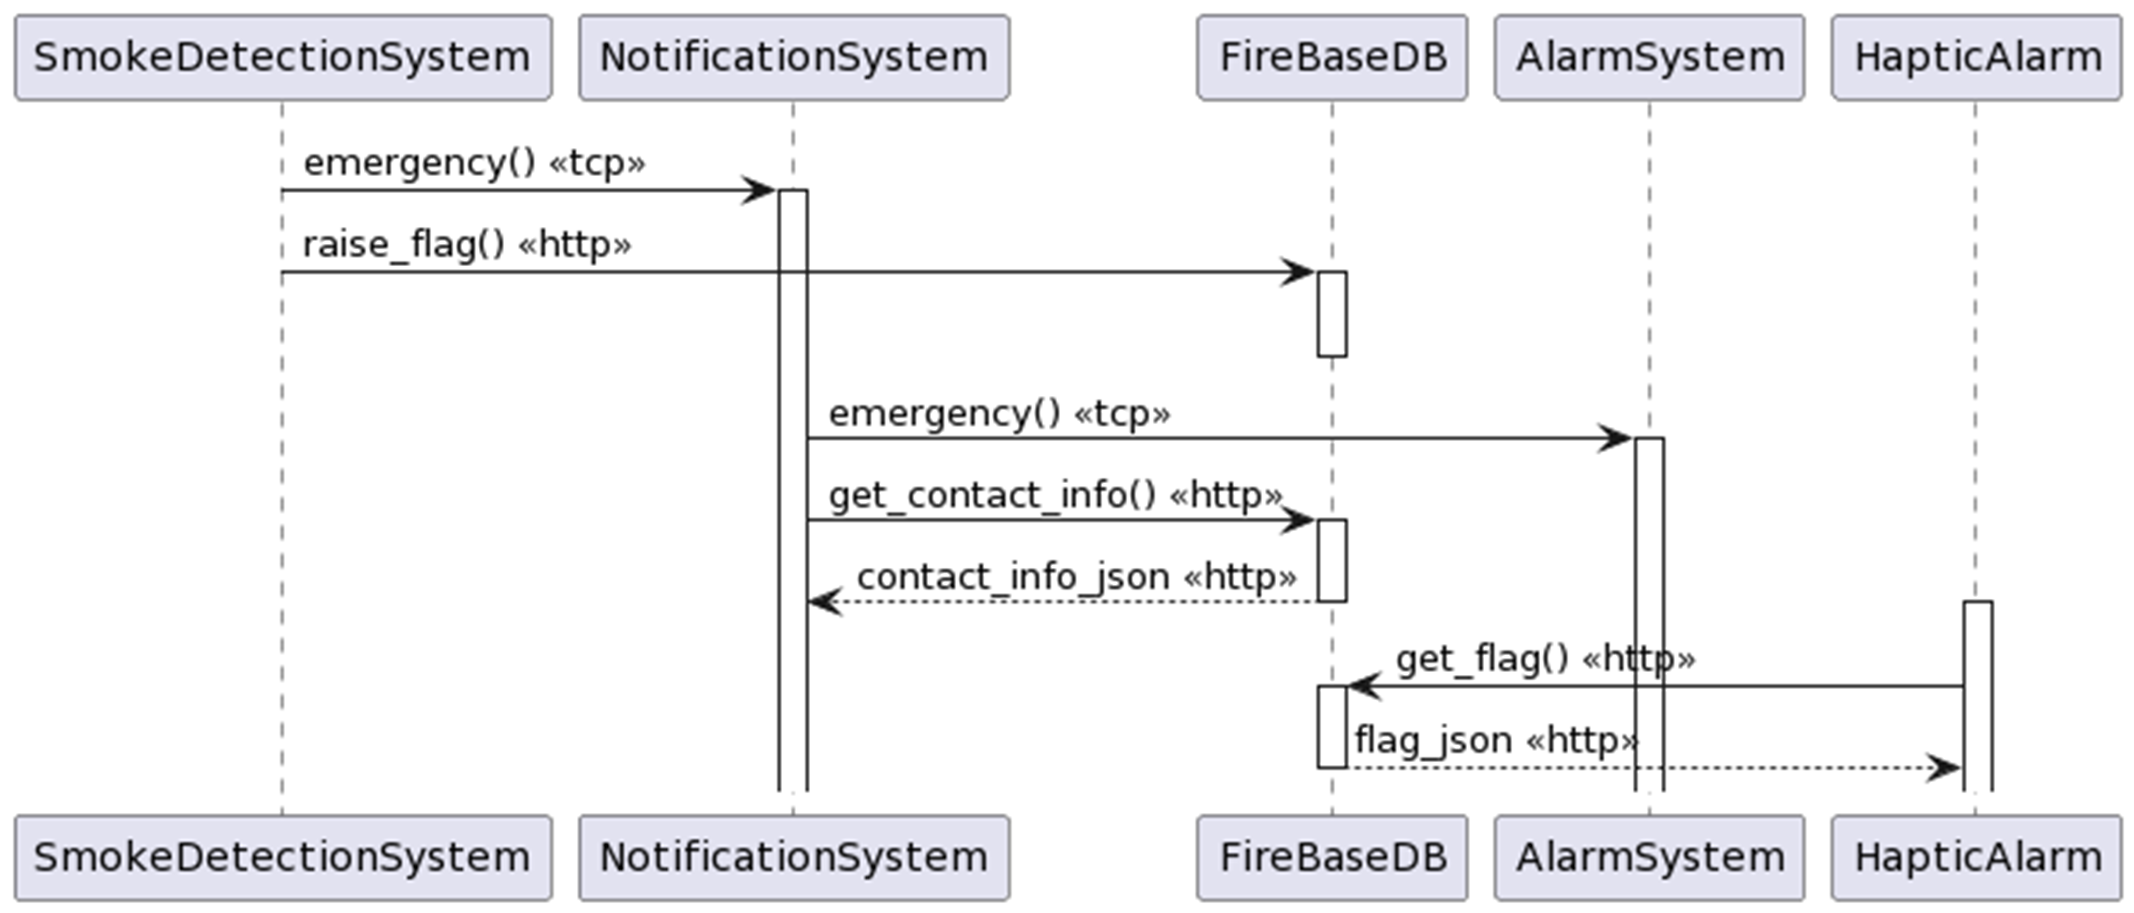
\includegraphics[width=\linewidth]{../assets/sequence/TriggerEmergencyUseCaseSequenceDiagram.png}
    \caption{Sequence diagram for the trigger emergency use case.}
\end{figure}

\subsubsection{Add New Contact Information Use Case}

This use case outlines the process by which users can add new contact information to the FANS database. Through the web
GUI, a user enters new contact details, such as phone numbers and email addresses, that the system can use to send
emergency notifications. Upon submission, these details are updated in the real-time database. The message sequence
diagram for this use case (not shown) illustrates the interactions between the user, the web GUI, and the database,
culminating in the notification system being updated with the new contact information. This ensures that the FANS can
reach the user through various channels in the event of an emergency, enhancing the system's effectiveness in
communicating critical alerts.

\begin{figure}[H]
    \centering
    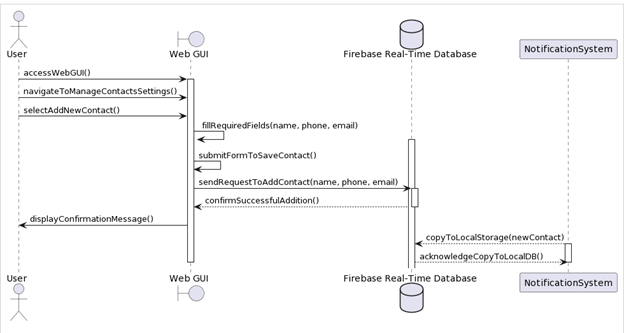
\includegraphics[width=\linewidth]{../assets/sequence/AddingNewContactInformationSequenceDiagram.png}
    \caption{Sequence diagram for the add contact info use case.}
\end{figure}

\subsubsection{Change Emergency Threshold Use Case}

Adjusting the smoke detection threshold is an essential feature that allows users to customize the sensitivity of the
FANS based on environmental conditions and personal preferences. This use case involves a user accessing the web GUI to
modify the threshold settings that determine when the smoke detection system should trigger an alert. The message
sequence diagram (not shown) visualizes the steps involved, from the user's interaction with the GUI to update the
threshold to the real-time database's role in storing this new setting. The smoke detection system then retrieves and
applies the updated threshold, ensuring that the FANS operates according to the user's specifications, balancing
sensitivity and false alarm minimization.

\begin{figure}[H]
    \centering
    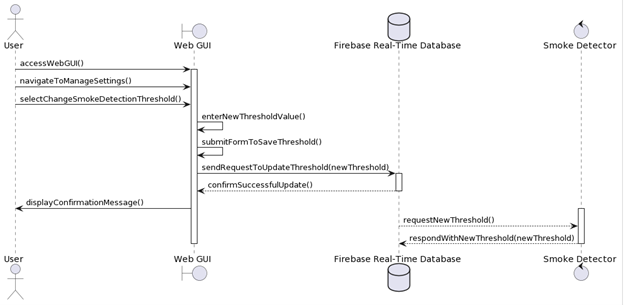
\includegraphics[width=\linewidth]{../assets/sequence/ChangingSmokeDetectionThresholdSequenceDiagram.png}
    \caption{Sequence diagram for the change threshold use case.}
\end{figure}

\subsubsection{Emergency Response Use Case}

This scenario highlights the FANS's capability to notify users in the event of a detected fire. Upon detecting a fire,
the notification system queries the cloud database for contact information and then sends out alerts via SMS and email
to all users. The message sequence diagram for this use case (provided above) captures the sequence of these
interactions, showcasing how the system ensures that occupants are informed and ready to address the emergency
promptly.

\begin{figure}[H]
    \centering
    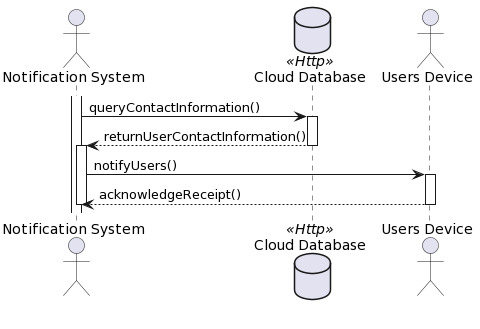
\includegraphics[width=\linewidth]{../assets/sequence/UserNotificationSequenceDiagram.png}
    \caption{Sequence diagram for the emergency response use case.}
\end{figure}

\subsection{Database Table Schema}

The FANS project will employ a Firebase Real-Time Database to store and manage data crucial for its operation. Given
the real-time nature of the FANS system, the choice of Firebase facilitates immediate updates and retrieval of data,
which is vital for emergency detection and notification. The data structure is designed to ensure efficient data
storage, retrieval, and management while supporting the scalability and real-time data processing requirements of the
system.

\begin{figure}[H]
    \centering
    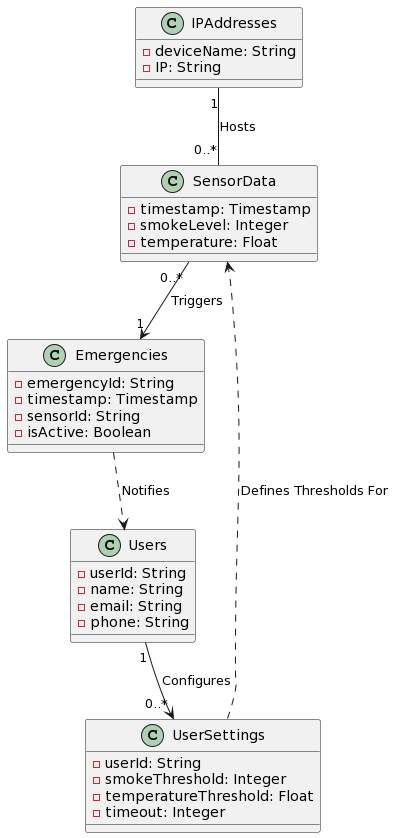
\includegraphics[width=3in]{../assets/class/DatabaseTableDesign.png}
    \caption{A visual of the FANS database design schema.}
\end{figure}

This schema optimizes the FANS system's performance by enabling efficient data storage, quick access to historical
data, and seamless integration between the system's components. The design also supports scalability, allowing for easy
addition of new sensors and users without significant alterations to the underlying database structure.
